% ===== 07_numerics =====
\section{数值验证与同条件控制比较}
\label{sec:num}
\label{sec:numerics}
\subsection{参数、指标口径与数值方法}
\label{sec:num:methods}
\begin{table}[htbp]
\centering\small
\setlength{\tabcolsep}{3.5pt}
\renewcommand{\arraystretch}{1.25}
\begin{threeparttable}
\caption{西安算例的参数与初始条件}
\label{tab:xian_initial_fit}
\begin{tabularx}{\linewidth}{@{}l>{\raggedright\arraybackslash}p{0.25\linewidth}>{\raggedright\arraybackslash}p{0.22\linewidth}>{\raggedright\arraybackslash}X@{}}
\toprule
符号 & 含义 & 取值或定义 & 来源或确定方式\\
\midrule
$N$ & 总人口 & \num{13163000} & 统计资料\cite{XianStat2021}\\
$\beta$ & 传播概率 & 0.1498 & 文献\cite{He2023TDINN}\\
$\gamma$ & 非隔离感染者移出率 & 0.2953 & 文献\cite{He2023TDINN}\\
$\delta_q$ & 隔离感染者移出率 & 0.3531 & 文献\cite{He2023TDINN}\\
$c_0$ & 常规接触率 & 12.8872 & 所采用控制函数在初始时刻的值\\
$q_0$ & 常规隔离率 & 0.3230 & 所采用控制函数在初始时刻的值\\
$I_0$ & 初始感染人数 & $\approx1.00659\times10^{-3}$ & 固定其余量后以最小二乘估计\\
$S_0$ & 初始易感人数 & $N-I_0$ & 总人口关系\\
$R(0)$ & 初始康复人数 & $0$ & 本文设定\\
$\eta$ & 非隔离感染人数上限 & $0.002N=\num{26326}$ & 代表性设计情景，见第\ref{sec:xian:threshold-scale}节\\
\bottomrule
\end{tabularx}
\begin{tablenotes}[flushleft]\footnotesize
\item 注：$c_0,\gamma,\delta_q$ 的时间单位为 $\mathrm d^{-1}$。仅 $I_0$ 为本文固定其他量后的初值估计；$S_0$ 不作独立估计。计算使用未取整的拟合结果；$\eta$ 为给定的设计阈值。
\end{tablenotes}
\end{threeparttable}
\end{table}

图\ref{fig:xian:observed-fit}与三策略比较、补充表\ref*{tab:sup:initial}使用统一归一化方程、DOP853 求解器和分量容差。日新增由相邻整数日累计量之差计算；仅隔离控制按常规、平台和退出后三阶段连接。观测窗口的初值比较及 TDINN 基准的容差敏感性见补充表\ref*{tab:sup:initial}；完整数值设置与历史程序对账见随文复现说明。

名义时间控制由状态积分预先确定，再输入完整仓室方程核查，不随数值积分的实时状态纠偏。
\subsection{仅隔离基准及参数权衡}
图\ref{fig:scenario1:single-sim}展示了上述三阶段过程。在图注所列参数下，控制于 $t_1\approx3.1754$ d 启动，此时 $S^*\approx708.3470$，隔离率由 $q_0$ 跳升至 $q_{\max}\approx0.7565$；随后感染人数保持在 $\eta=38.15$，直至 $S$ 降至 $S_c\approx175.1602$，并于 $t_2\approx9.0780$ d 恢复常规隔离率。对应的控制持续时间约为 $5.9026$ d，而常规控制的感染峰值约为 $300.4$，出现在 $6.7$ d 附近。基准数值积分中控制区间上的最大阈值偏差为 $1.07\times10^{-7}$，支持数值轨迹与解析结果的一致性。
\begin{figure}[htbp]
\centering
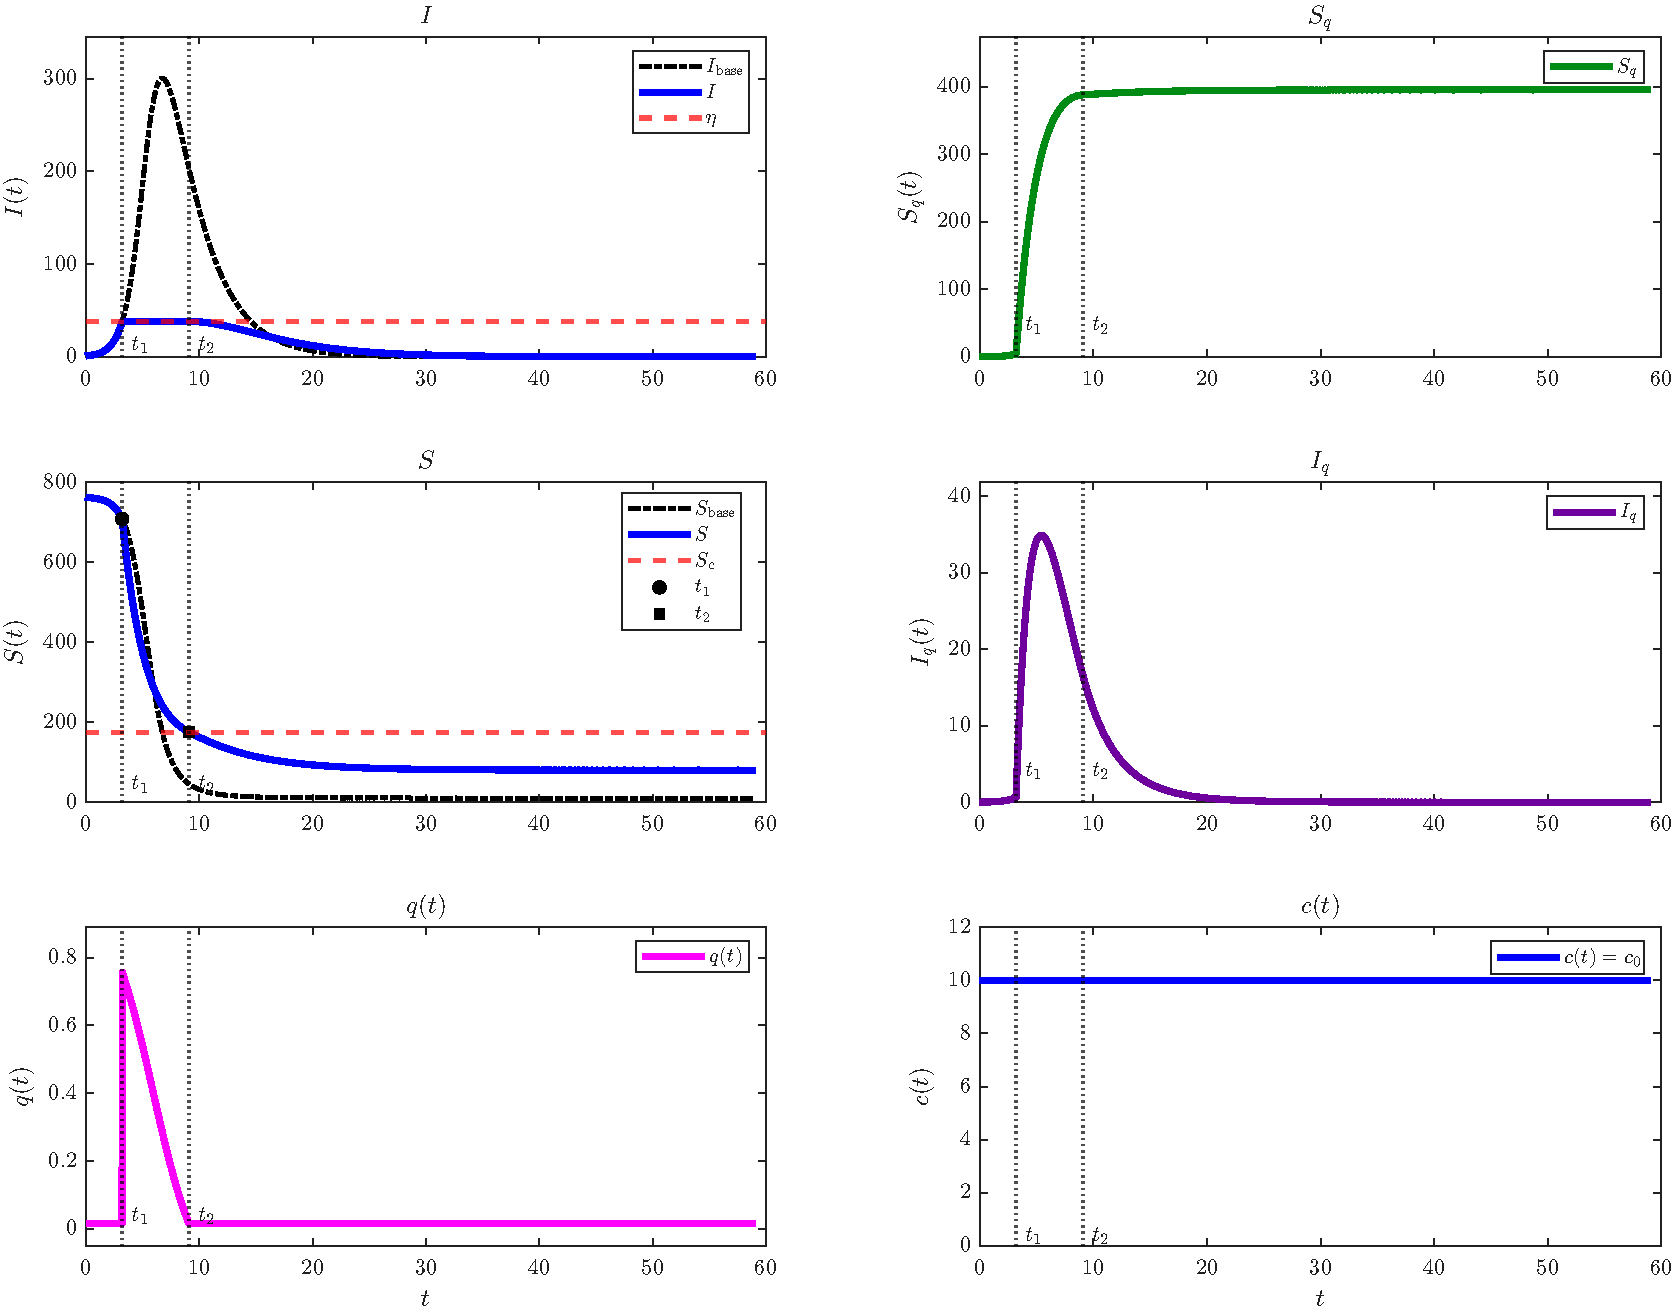
\includegraphics[width=0.7\textwidth]{figures/optimal_control_with_quarantine_panels.pdf}
\caption{仅隔离阈值控制与常规控制的时间轨迹。参数为 $N=763$、$S_0=762$、$I_0=1$、$S_q(0)=I_q(0)=R(0)=0$、$\beta=0.155$、$c_0=10\ \mathrm d^{-1}$、$q_0=0.01526$、$\gamma=\delta_q=0.3504\ \mathrm d^{-1}$、$\eta=0.05N=38.15$。此处的阈值比例用于说明解析结果，不作具体 ICU 容量换算。阈值控制在 $[t_1,t_2]$ 内维持 $I=\eta$，$q_c$ 从启动最大值下降至 $q_0$；$c(t)$ 始终为 $c_0$。横轴为自初始时刻起的天数。}
\label{fig:scenario1:single-sim}
\end{figure}


图\ref{fig:scenario1:single-sim}说明仅隔离策略的完整过程。本节比较常规接触率和感染阈值对多个结果指标的影响，参数取值见各图图注。不同 $c_0$ 对应不同的常规接触水平，每条轨迹内仍保持 $c(t)\equiv c_0$。当 $\eta=0.05N$ 时，控制触发边界为
\[
c_{0,\min}(0.05N)\approx3.3270.
\]
仅在满足触发条件的参数范围内计算控制指标。补充表\ref*{tab:sup:baseline}分别列出固定 $\eta/N=5\%$ 与固定 $c_0=10$ 的结果；控制轨迹见图\ref{fig:baseline:q-joint}，多指标变化见图\ref{fig:scenario1_summary_c0}、\ref{fig:scenario1_summary_eta}。


\begin{figure}[htbp]
\centering
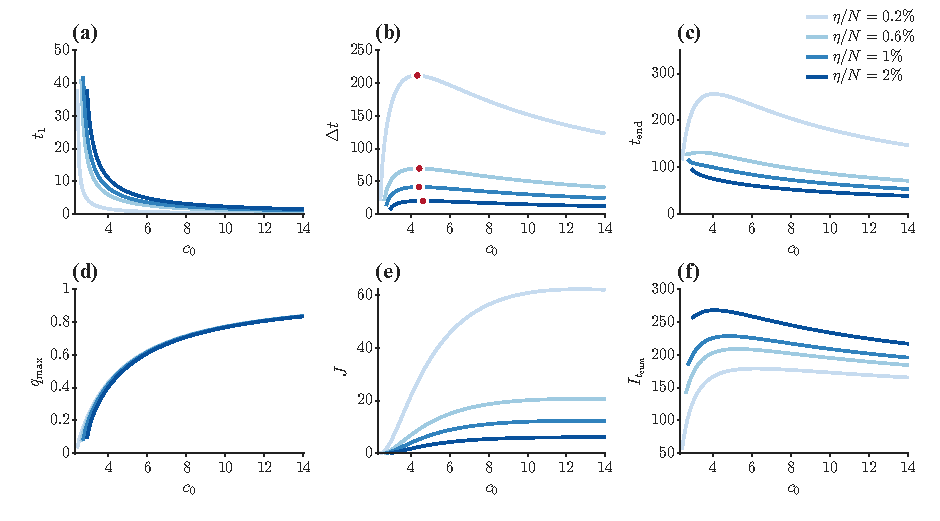
\includegraphics[width=\textwidth]{figures/layout_v5/c0_sensitivity_selected_eta.pdf}
\caption{不同阈值比例下各指标随 $c_0$ 的变化。固定 $N=763,S_0=762,I_0=1,\beta=0.155,\gamma=0.3504\ \mathrm d^{-1},q_0=0.01526$，$\eta/N=0.2\%,0.6\%,1\%,2\%$，红色圆点表示 $\Delta t$ 的数值极大值。}
\label{fig:scenario1_summary_c0}
\end{figure}


\begin{figure}[htbp]
\centering
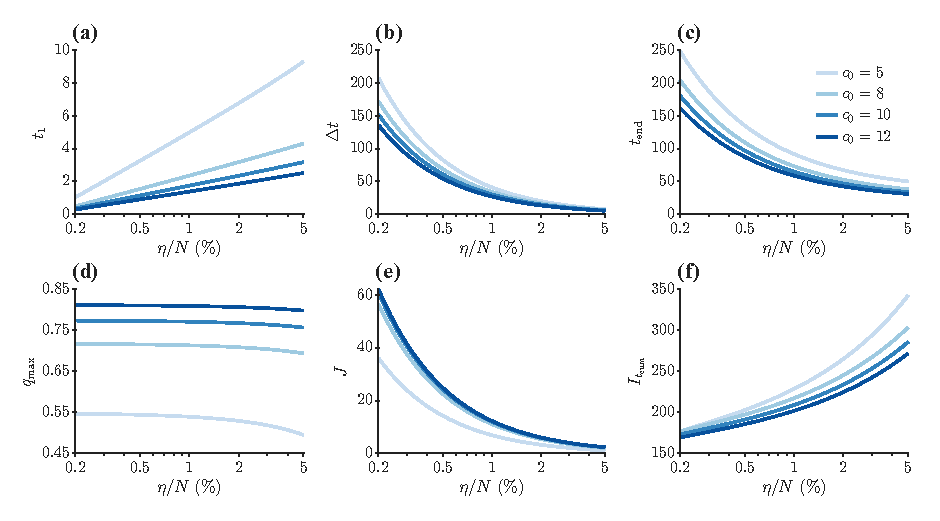
\includegraphics[width=\textwidth]{figures/layout_v5/eta_sensitivity_selected_c0.pdf}
\caption{不同常规接触率下各指标随 $\eta/N$ 的变化。固定 $N=763,S_0=762,I_0=1,\beta=0.155,\gamma=0.3504\ \mathrm d^{-1},q_0=0.01526$，$c_0=5,8,10,12$。}
\label{fig:scenario1_summary_eta}
\end{figure}


%\clearpage

图~\ref{fig:baseline:q-joint}(a) 中，$c_0=4$ 时 $q_{\max}=0.3413<\qinf\approx0.4083$，不存在内部拐点；$c_0=5,8,10,12$ 时均存在唯一内部拐点。图~\ref{fig:baseline:q-joint}(b) 中，各拐点对应的隔离率相同，但启动时间和控制持续时间随阈值改变。

由表~\ref*{tab:sup:baseline} 和图~\ref{fig:scenario1_summary_c0}，增大 $c_0$ 会提高启动点 $S^*$ 和最大隔离率 $q_{\max}$，并使启动时间提前。控制时长在所考察范围内先增加后减小。例如，$\eta/N=5\%$ 时，
\[
\Delta t(3.3470)=2.0432,\qquad
\Delta t(5)=7.5778,\qquad
\Delta t(12)=5.3007\ {\rm d}.
\]
相应的数值极大值位于 $c_0\approx5.1$，约为 $7.5788$ 天。对于 $\eta/N=0.2\%,0.6\%,1\%,2\%$，极大值位置分别约为 $c_0=4.3,4.4,4.4,4.6$，对应时长为 $211.5435,69.8417,41.5169,20.2813$ 天。

表~\ref*{tab:sup:baseline} 和图~\ref{fig:scenario1_summary_eta} 表明，增大 $\eta$ 会推迟控制启动、降低 $q_{\max}$，并缩短阈值控制期。当 $c_0=10$、$\eta/N$ 从 $0.2\%$ 增至 $2\%$ 时，
\[
\Delta t:152.0574\to15.0431,\qquad
t_{\rm end}:180.5821\to46.8029,
\]
\[
J:60.8005\to5.8888,\qquad
\Itcum:173.0314\to233.7810.
\]
在这一参数范围内，提高阈值缩短了阈值控制期和清零时间，降低了控制成本，但增加了累计感染。图~\ref{fig:scenario1_heatmaps_c0_eta} 给出这些指标在 $(\eta/N,c_0)$ 平面上的变化。触发边界 $c_{0,\min}(\eta)$ 随 $\eta$ 增大而升高；其下方的常规感染峰值低于阈值，无需启动加强隔离。

\FloatBarrier
\subsection{两组参数下的四种分配}
\label{sec:joint:compare-numerics}
% BEGIN JOINT_EXTRA:comparison
在同一完整初值、阈值和退出目标下，比较仅减少接触、显式族 $\alpha=0.5$、仅隔离和类内最小二次成本四种分配。基准参数沿用图\ref{fig:scenario1:single-sim}，西安参数沿用第\ref{sec:xian}节的未取整初值；两组均取 $w_c=1,w_q=2$。结果见表\ref{tab:joint:compare}及图\ref{fig:joint:compare}。

基准参数下，类内最小成本为 $J_{\min}\approx2.1183$，控制时长约为 $7.7536$ d；仅隔离的对应值为 $2.2236$ 和 $5.9026$ d。总累计新增感染分别约为 $306.6$ 和 $285.7$ 人。相对仅隔离，成本降低约 $4.7\%$，控制时间增加约 $31.4\%$，总累计新增感染增加约 $7.3\%$。最低成本分配的控制时间更长、累计新增感染更多、控制期新增隔离易感者更少，与式\eqref{eq:joint:cumulative}--\eqref{eq:joint:quarantine}的排序一致。

两组参数下，最低成本分配都分为前后两段。基准和西安参数的启动状态分别为 $S^*/S_c\approx4.044$ 和 $4.378$，均大于 $S_{\rm sw}/S_c\approx2.265$ 和 $2.548$。由命题\ref{prop:joint:global-structure}，任一类内最小成本可测控制在 $S_c<S<S_{\rm sw}$ 上几乎处处同时使用两种措施；$S>S_{\rm sw}$ 时该命题只说明仅隔离是局部最小点。对 $w_c=1,w_q=2$ 比较全部候选后，数值结果显示 $S>S_{\rm sw}$ 上的全局最小点就是仅隔离，切换发生在 $S=S_{\rm sw}$ 处且分配连续；退出时两种控制回到常规水平（权重的影响见第\ref{sec:joint:weights-numerics}节）。基准参数下，仅隔离段约为 $1.61$ d，占控制时长的 $21\%$，但 $S$ 在该段的下降占平台期总下降的 $58\%$；此后接触率最大降低约 $19.8\%$。西安参数下相应为 $25.46$ d、$23\%$、$54\%$ 和 $28.2\%$。平台期成本和控制时长都是关于 $S$ 的积分，两种分配在 $S\ge S_{\rm sw}$ 一段的贡献相同，表\ref{tab:joint:compare}中二者 $J$ 与 $\Delta t$ 的差别只来自 $S_c<S<S_{\rm sw}$ 一段。在这一段，最低成本分配取 $c_c(S)<c_0$，由 $\dot S=-(\eta/N)[c_c(S)S-c_0\bar S]$，相较仅隔离，$S$ 下降较慢，控制时间因而延长；隔离强度相应降低，二次成本减小。

感染人数上限约束的是 $I$，不是 $I+I_q$。在各自 $[0,t_{\rm end}]$ 上，基准参数下仅隔离、最低成本分配与仅减少接触的 $\max(I+I_q)/\eta$ 分别约为 $1.92$、$1.89$ 和 $1.02$；西安参数下相应为 $4.73$、$4.73$ 和 $1.46$。西安参数下，仅隔离与最低成本分配的这一峰值都出现在启动后约 $7.62$ d，此时两者仍处于分配相同的 $S>S_{\rm sw}$ 一段，故峰值相同；基准参数下仅隔离的峰值出现在两者分开之后，最低成本分配的峰值略低。这些是现存感染人数，不是医疗或 ICU 占用；图\ref{fig:joint:compare}(c)中的水平线 $1$ 只作归一化参照。

\begingroup
\begin{table}[htbp]
\centering\small
\setlength{\tabcolsep}{3.5pt}
\renewcommand{\arraystretch}{1.25}
\begin{threeparttable}
\caption{相同阈值与启动、退出要求下四种分配的结果（$w_c=1,w_q=2$）}
\label{tab:joint:compare}
\begin{tabularx}{\linewidth}{@{}>{\raggedright\arraybackslash}Xccccc@{}}
\toprule
分配 & \shortstack{控制时长\\$\Delta t$（d）} & \shortstack{清零时刻\\$t_{\rm end}$（d）} & \shortstack{总累计\\新增感染} & \shortstack{控制期新增\\隔离易感者} & $J$（d）\\
\midrule
\multicolumn{6}{@{}l}{基准参数：$N=763$，$\eta=0.05N$；新增人数单位为人}\\
仅减少接触 & 36.26 & 64.13 & 628.6 & 40.9 & 11.9390\\
显式族 $\alpha=0.5$ & 9.24 & 37.11 & 323.4 & 346.2 & 2.5462\\
仅隔离 & 5.90 & 33.77 & 285.7 & 383.9 & 2.2236\\
类内最小成本 & 7.75 & 35.62 & 306.6 & 363.0 & 2.1183\\
\midrule
\multicolumn{6}{@{}l}{西安参数：$\eta=0.002N$；新增人数单位为 $10^6$ 人}\\
仅减少接触 & 308.79 & 481.83 & 3.8566 & 6.5004 & 109.3648\\
显式族 $\alpha=0.5$ & 124.57 & 297.60 & 2.6390 & 7.7180 & 44.5286\\
仅隔离 & 85.07 & 258.10 & 2.3779 & 7.9791 & 40.7686\\
类内最小成本 & 108.81 & 281.84 & 2.5348 & 7.8222 & 38.0209\\
\bottomrule
\end{tabularx}
\begin{tablenotes}[flushleft]\footnotesize
\item 注：每组沿用同一完整初值、首次上升至 $I=\eta$ 的启动规则和 $S=S_c$ 的退出目标，各自恢复常规后在 $I$ 下降至 $1$ 时终止。累计新增感染不包含初始感染者；新增隔离易感者只统计控制期。$J$ 为式\eqref{eq:cost:J}的二次成本，不由线性 $J_c,J_q$ 加总。西安参数及未取整初值见第\ref{sec:xian}节；表内单位和显示精度按行组区分。
\end{tablenotes}
\end{threeparttable}
\end{table}
\endgroup
% END JOINT_EXTRA:comparison

在同一全市人口、未取整拟合初值及 $\eta=0.002N$ 下，第\ref{sec:joint:compare-numerics}节又比较了四种阈值分配（表\ref{tab:joint:compare}）。类内最小成本从仅隔离的 $40.7686$ 降至 $38.0209$，控制时长由 $85.07$ 延长至 $108.81$ d，总累计新增感染由约 $2.3779\times10^6$ 增至 $2.5348\times10^6$。相对变化分别约为成本 $-6.7\%$、控制时长 $+27.9\%$、总累计新增感染 $+6.6\%$。因此，这里的成本降低不伴随感染指标同时改善。
\begin{figure}[htbp]
\centering
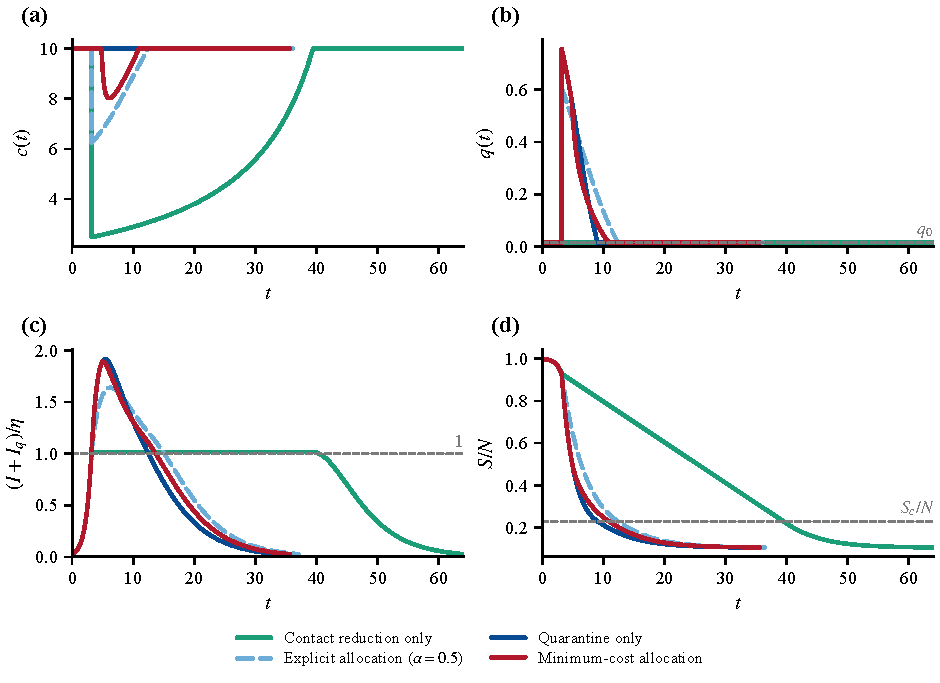
\includegraphics[width=\textwidth]{figures/joint_v2/joint_compare_baseline.pdf}
\caption{基准参数下相同启动与退出要求的四种分配（$N=763$，$\eta=0.05N$，$w_c=1,w_q=2$）。(a) 接触率；(b) 隔离率；(c) 现存感染人数与阈值之比 $(I+I_q)/\eta$；(d) 社区易感者比例。各轨迹画至自身的动态清零时刻，横轴 $t$ 为自共同初始时刻起的天数。控制跳变按分段数据绘制；(c) 的水平 $1$ 为归一化参照，不是本文对总感染现患人数的约束。}
\label{fig:joint:compare}
\end{figure}

\FloatBarrier
% TODO（阶段4e-3）：迁入的西安数值段与本节表格仍有重复，按批准范围精简。
\subsection{能力限制下的可行性与受限分配}
\label{sec:joint:capacity-numerics}
% BEGIN JOINT_EXTRA:capacity
\def\jointcapacitypostexitdays{1}
图\ref{fig:joint:capacity}将能力平面分成至少一种单控制可行、两种单控制均不可行但联合可行、规定触发状态下不可行三个区域。仅隔离可行要求 $q_{\rm cap}\ge q_{\max}$，仅减少接触可行要求 $c_{\min}\le c_0S_c/S^*$；二者均不成立时由式\eqref{eq:joint:feasibility}判断联合可行性，边界等号归入可行侧。灰色区域的不可行只针对在 $I$ 首次达到 $\eta$ 时启动、在 $S=S_c$ 退出的平台控制。

基准参数代表点取 $c_{\min}/c_0=0.5$、$q_{\rm cap}=0.6$。仅隔离需要 $q_{\max}\approx0.756$，仅减少接触需要把接触率降低约 $75.3\%$，两者均超出能力限制，联合控制可行。受限类内最小成本约为 $2.3611$，控制时长约为 $8.34$ d，比无额外能力限制时分别增加约 $11.5\%$ 和 $7.5\%$。西安代表点取 $c_{\min}/c_0=0.5$、$q_{\rm cap}=0.75$，相应为 $41.6166$ 和 $116.75$ d，增幅约为 $9.5\%$ 和 $7.3\%$。

图\ref{fig:joint:capacity}(c)给出基准代表点的时间控制。启动后约 $1.94$ d 内，隔离比例停在上限 $0.6$，接触率同时降低，降幅由启动时的约 $39.1\%$ 随 $S$ 下降而减小；$S$ 降至 $(1-q_0)S_c/(1-q_{\rm cap})\approx2.462S_c$ 时，仅隔离已能维持平台，接触率回到 $c_0$。随后经过约 $0.26$ d 的仅隔离段，$S<S_{\rm sw}$ 后两种措施同时使用直至退出。在 $S\le(1-q_0)S_c/(1-q_{\rm cap})$ 上，无额外限制时的逐状态最小点满足两项能力限制，因而也是受限问题的逐状态最小点，数值核查显示同一 $S$ 处两者的 $c_c(S)$、$q_c(S)$ 相同。这里的一致只指同一易感者状态下的控制：受限分配到达同一 $S$ 的时刻较晚，$I_q$、$S_q$ 等状态也不同，并非相同时刻的完整轨迹相同。由于 $J$ 与 $\Delta t$ 都是关于 $S$ 的积分，能力限制只改变启动后的前一段分配，二者的增加都来自这一段。西安代表点的结构相同，隔离比例停在上限约 $30.38$ d。有能力限制时，可达到的最短和最长控制时长由实际允许区间的上下界给出，不再对应两种单控制。
% END JOINT_EXTRA:capacity

\begin{figure}[htbp]
\centering
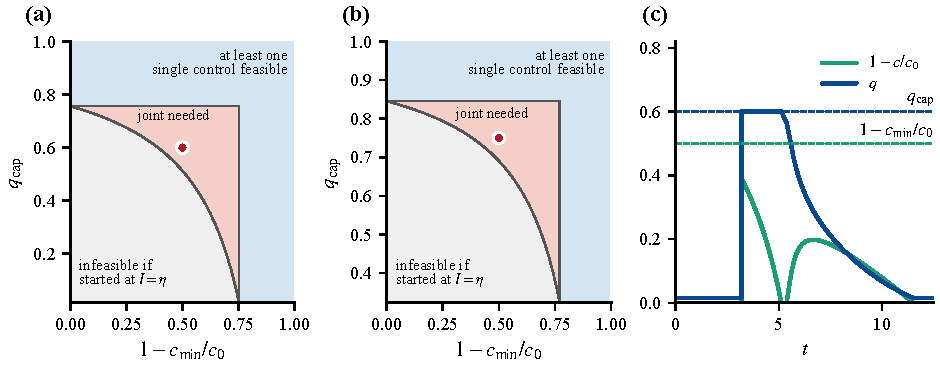
\includegraphics[width=\textwidth]{figures/joint_v2/joint_capacity.pdf}
\caption{能力限制下的可行区域与代表轨迹。(a) 基准参数；(b) 西安参数。横轴为最大接触减少比例 $1-c_{\min}/c_0$，纵轴为隔离比例上限 $q_{\rm cap}$；灰色、浅红色、浅蓝色分别表示规定触发状态下不可行、需联合控制、至少一种单控制可行，边界归入可行侧。红点为代表能力组合。(c) 基准代表点的受限最低二次成本分配，绘至名义退出后\jointcapacitypostexitdays{}天，横轴 $t$ 的单位为天。}
\label{fig:joint:capacity}
\end{figure}

\FloatBarrier
\subsection{成本权重与分配结构}
\label{sec:joint:weights-numerics}
% BEGIN JOINT_EXTRA:phase
为比较分配结构，固定 $w_c=1$ 并改变 $r=w_q/w_c$；其余参数及状态固定时，权重对逐状态最小点的影响仅通过比值 $r$。图\ref{fig:joint:phase}给出 $r\in[0.1,20]$ 上 $161$ 个对数等距取值的结果，颜色 $y=(1-c_c^*/c_0)/(1-S_c/S)$ 是接触减少相对于仅减少接触端点的比例，$y=0$ 与 $y=1$ 分别对应两种单控制（隔离强度不是 $1-y$）。全局切换点由端点与内部驻点的成本比较确定；命题\ref{prop:joint:global-structure}中的 $S_{\rm sw}$ 只给出端点的局部性质，基准和西安参数分别约为 $2.265S_c$ 和 $2.548S_c$。

在所计算的 $161$ 个网格点上，基准参数直到网格点 $r\approx3.13$、西安参数直到网格点 $r\approx2.65$，各点的全局切换点都与 $S_{\rm sw}$ 重合且分配连续：$S>S_{\rm sw}$ 时取仅隔离，$S<S_{\rm sw}$ 时两种措施同时使用。默认 $r=2$ 不是网格点；第\ref{sec:joint:compare-numerics}节在 $r=2$ 下单独完成的候选比较同样给出 $S=S_{\rm sw}$ 处的连续切换。从相邻的网格点 $r\approx3.24$（基准）和 $r\approx2.74$（西安）起，仅隔离段在 $S$ 降至 $S_{\rm sw}$ 之前结束：$S$ 略大于 $S_{\rm sw}$ 时仅隔离仍是局部最小点，但内部的另一局部最小点成本更低。在其后的网格点上，切换点随 $r$ 增大移向启动状态，接触率在切换处由 $c_0$ 跳到内部值；例如 $r\approx4.98$ 时，基准和西安的切换点约为 $2.544S_c$ 和 $3.367S_c$，接触率分别跳至约 $0.539c_0$ 和 $0.369c_0$。出现仅隔离段的最大网格点为 $r\approx13.00$（基准）和 $7.41$（西安），从 $r\approx13.44$ 和 $7.66$ 起，整个平台期不再出现仅隔离段。相邻网格点显示了上述两处结构变化，但未进一步确定连续权重下的精确转折位置或证明其唯一性。靠近退出时，各 $r$ 下的 $y$ 趋于 $r/(1+r)$，与命题\ref{prop:joint:terminal-allocation}一致。改变 $r$ 即改变成本标准，不同 $r$ 下的 $J$ 不直接比较。
% END JOINT_EXTRA:phase

\begin{figure}[htbp]
\centering
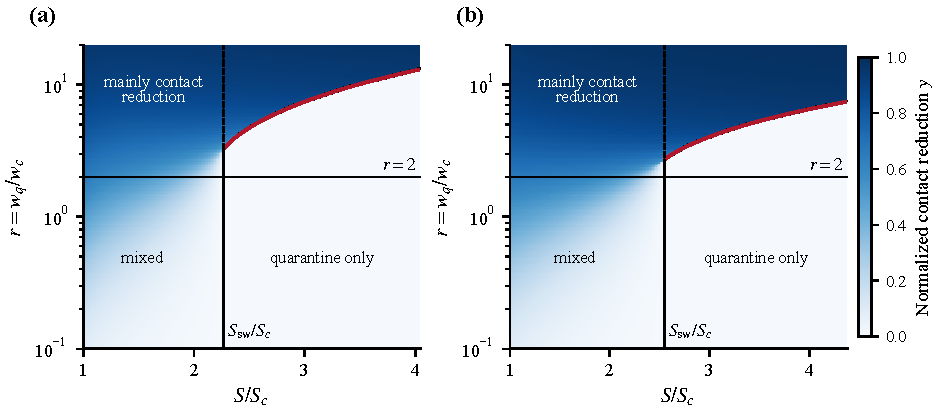
\includegraphics[width=\textwidth]{figures/joint_v2/joint_phase_weights.pdf}
\caption{固定 $w_c=1$、改变 $r=w_q/w_c$ 时的类内最低二次成本分配。(a) 基准参数；(b) 西安参数。颜色为 $y=(1-c_c^*/c_0)/(1-S_c/S)$，$y=0$ 为仅隔离，$y=1$ 为仅减少接触。竖直线位于局部阈值 $S_{\rm sw}/S_c$，其实线段与红色曲线为数值比较得到的全局切换边界，红色曲线处接触率跳变；水平点线为默认 $r=2$。沿控制时间，$S$ 从右向左减小。}
\label{fig:joint:phase}
\end{figure}

\FloatBarrier
% BEGIN JOINT_EXTRA:duration
\subsection{成本—控制时长关系}
\label{sec:joint:duration-numerics}
图\ref{fig:joint:frontier}给出基准参数下 $470$ 个经数值核查的乘子解，每个解报告实际 $\Delta t$ 与原二次成本 $J$。注记\ref{rem:joint:duration-constraint}给出的是充分条件：取得时长匹配的乘子解 $c_\kappa$ 时，它是约束 $\Delta t=\Delta t[c_\kappa]$ 下的类内最小成本控制。两种单控制之间的每个时长都可由允许控制实现，但计算点之间的时长未逐一取得匹配乘子，这些时长上的最低成本未由此确定。

在当前参数下，计算点显示最低成本附近 $J$ 对 $\Delta t$ 不敏感。若要求 $\Delta t\le T$ 且 $\Delta t[c_0]\le T\le\Delta t[c_c^*]$，仅隔离满足这一限制，故成本下界为无额外时长限制的最低二次成本 $J_{\min}=J[c_c^*]$，上界为仅隔离的实际二次成本 $J[c_0]$。两个时长端点约为 $5.90$ 和 $7.75$ d，而 $J[c_0]\approx1.05J_{\min}$ 仅作显示近似；$\kappa\ge0$ 的计算点均落在上述实际成本范围内。$\kappa<0$ 一侧，满足 $J\le1.10J_{\min}$ 的计算点中最大时长约为 $11.09$ d，下一个计算点（$11.40$ d）约为 $1.12J_{\min}$；$11.09$ d 不是精确的临界时长。仅减少接触端点（$36.26$ d）的 $J$ 约为 $5.64J_{\min}$。$\kappa<0$ 的解对应时长下限，由式\eqref{eq:joint:quarantine}等价于限制控制期新增隔离易感者人数；若只考虑 $J$ 与 $\Delta t$，这些解的两项都大于最低成本点，因此整条曲线不是同时最小化二者的效率前沿。显式 $\alpha$ 族属于同一允许控制类，只作对照。

\begin{figure}[htbp]
\centering
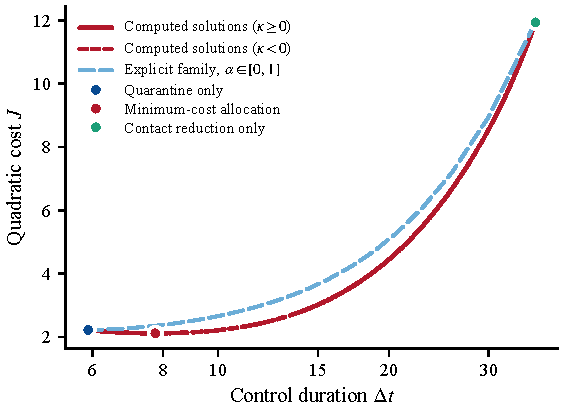
\includegraphics[width=0.6\textwidth]{figures/joint_v2/joint_frontier_baseline.pdf}
\caption{基准参数下二次成本与控制持续时间的关系。红色曲线连接已核查的 $J+\kappa\Delta t$ 最小化解，实线与短虚线分别对应 $\kappa\ge0$ 和 $\kappa<0$；连线不表示中间时长已有匹配乘子。浅蓝虚线为显式 $\alpha$ 族，圆点为两种单控制与无时长限制的最低成本分配。横轴为对数坐标，$\Delta t$ 与 $J$ 的单位均为天。}
\label{fig:joint:frontier}
\end{figure}
% END JOINT_EXTRA:duration

\FloatBarrier

